%Colocar Figuras e cógigo nos anexos
\section{Anexos}
\subsection{Anexo 1}
	\begin{figure}[!h]
		\centering
		\caption{Ilustração do workflow do Montage}
			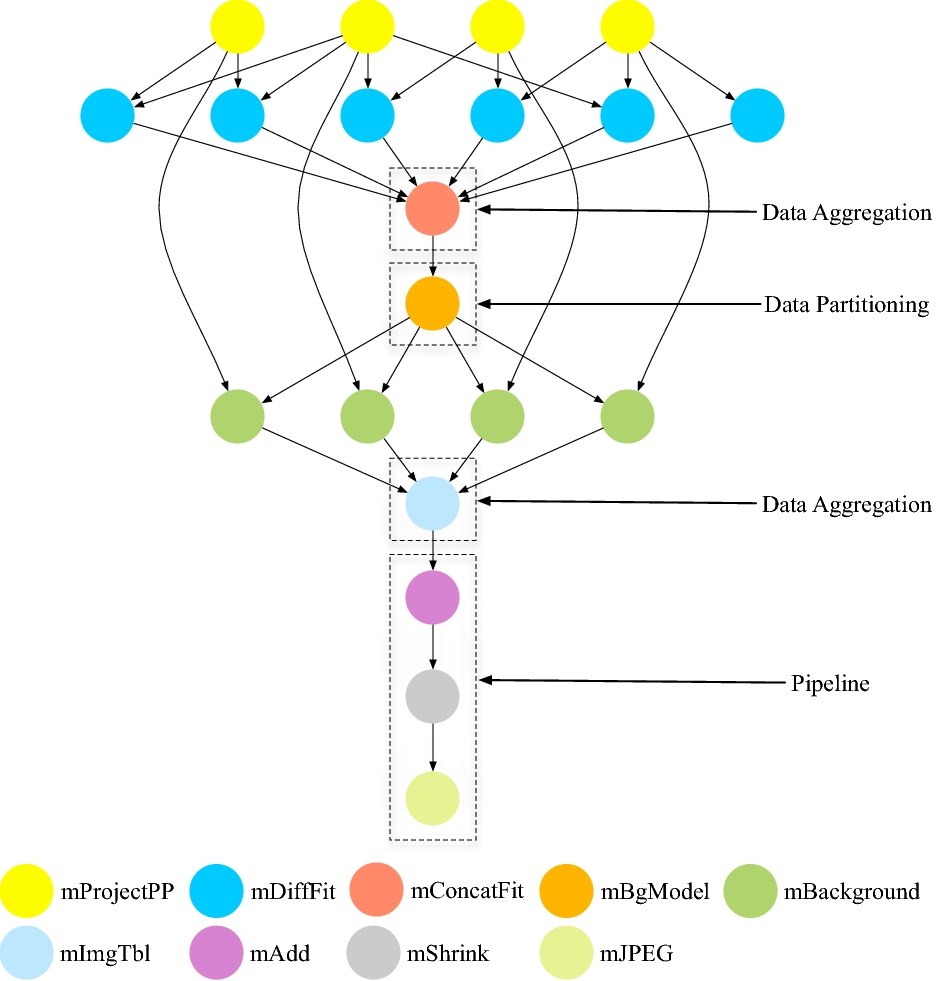
\includegraphics[width=1.1\textwidth]{img/Montage.jpg}
		\label{Anexo 1}
	\end{figure}



\subsection{Anexo 2}
\begin{landscape}
	\begin{figure}
		\centering
		\caption{Representação Gráfica do Montage usando Redes de Petri}
		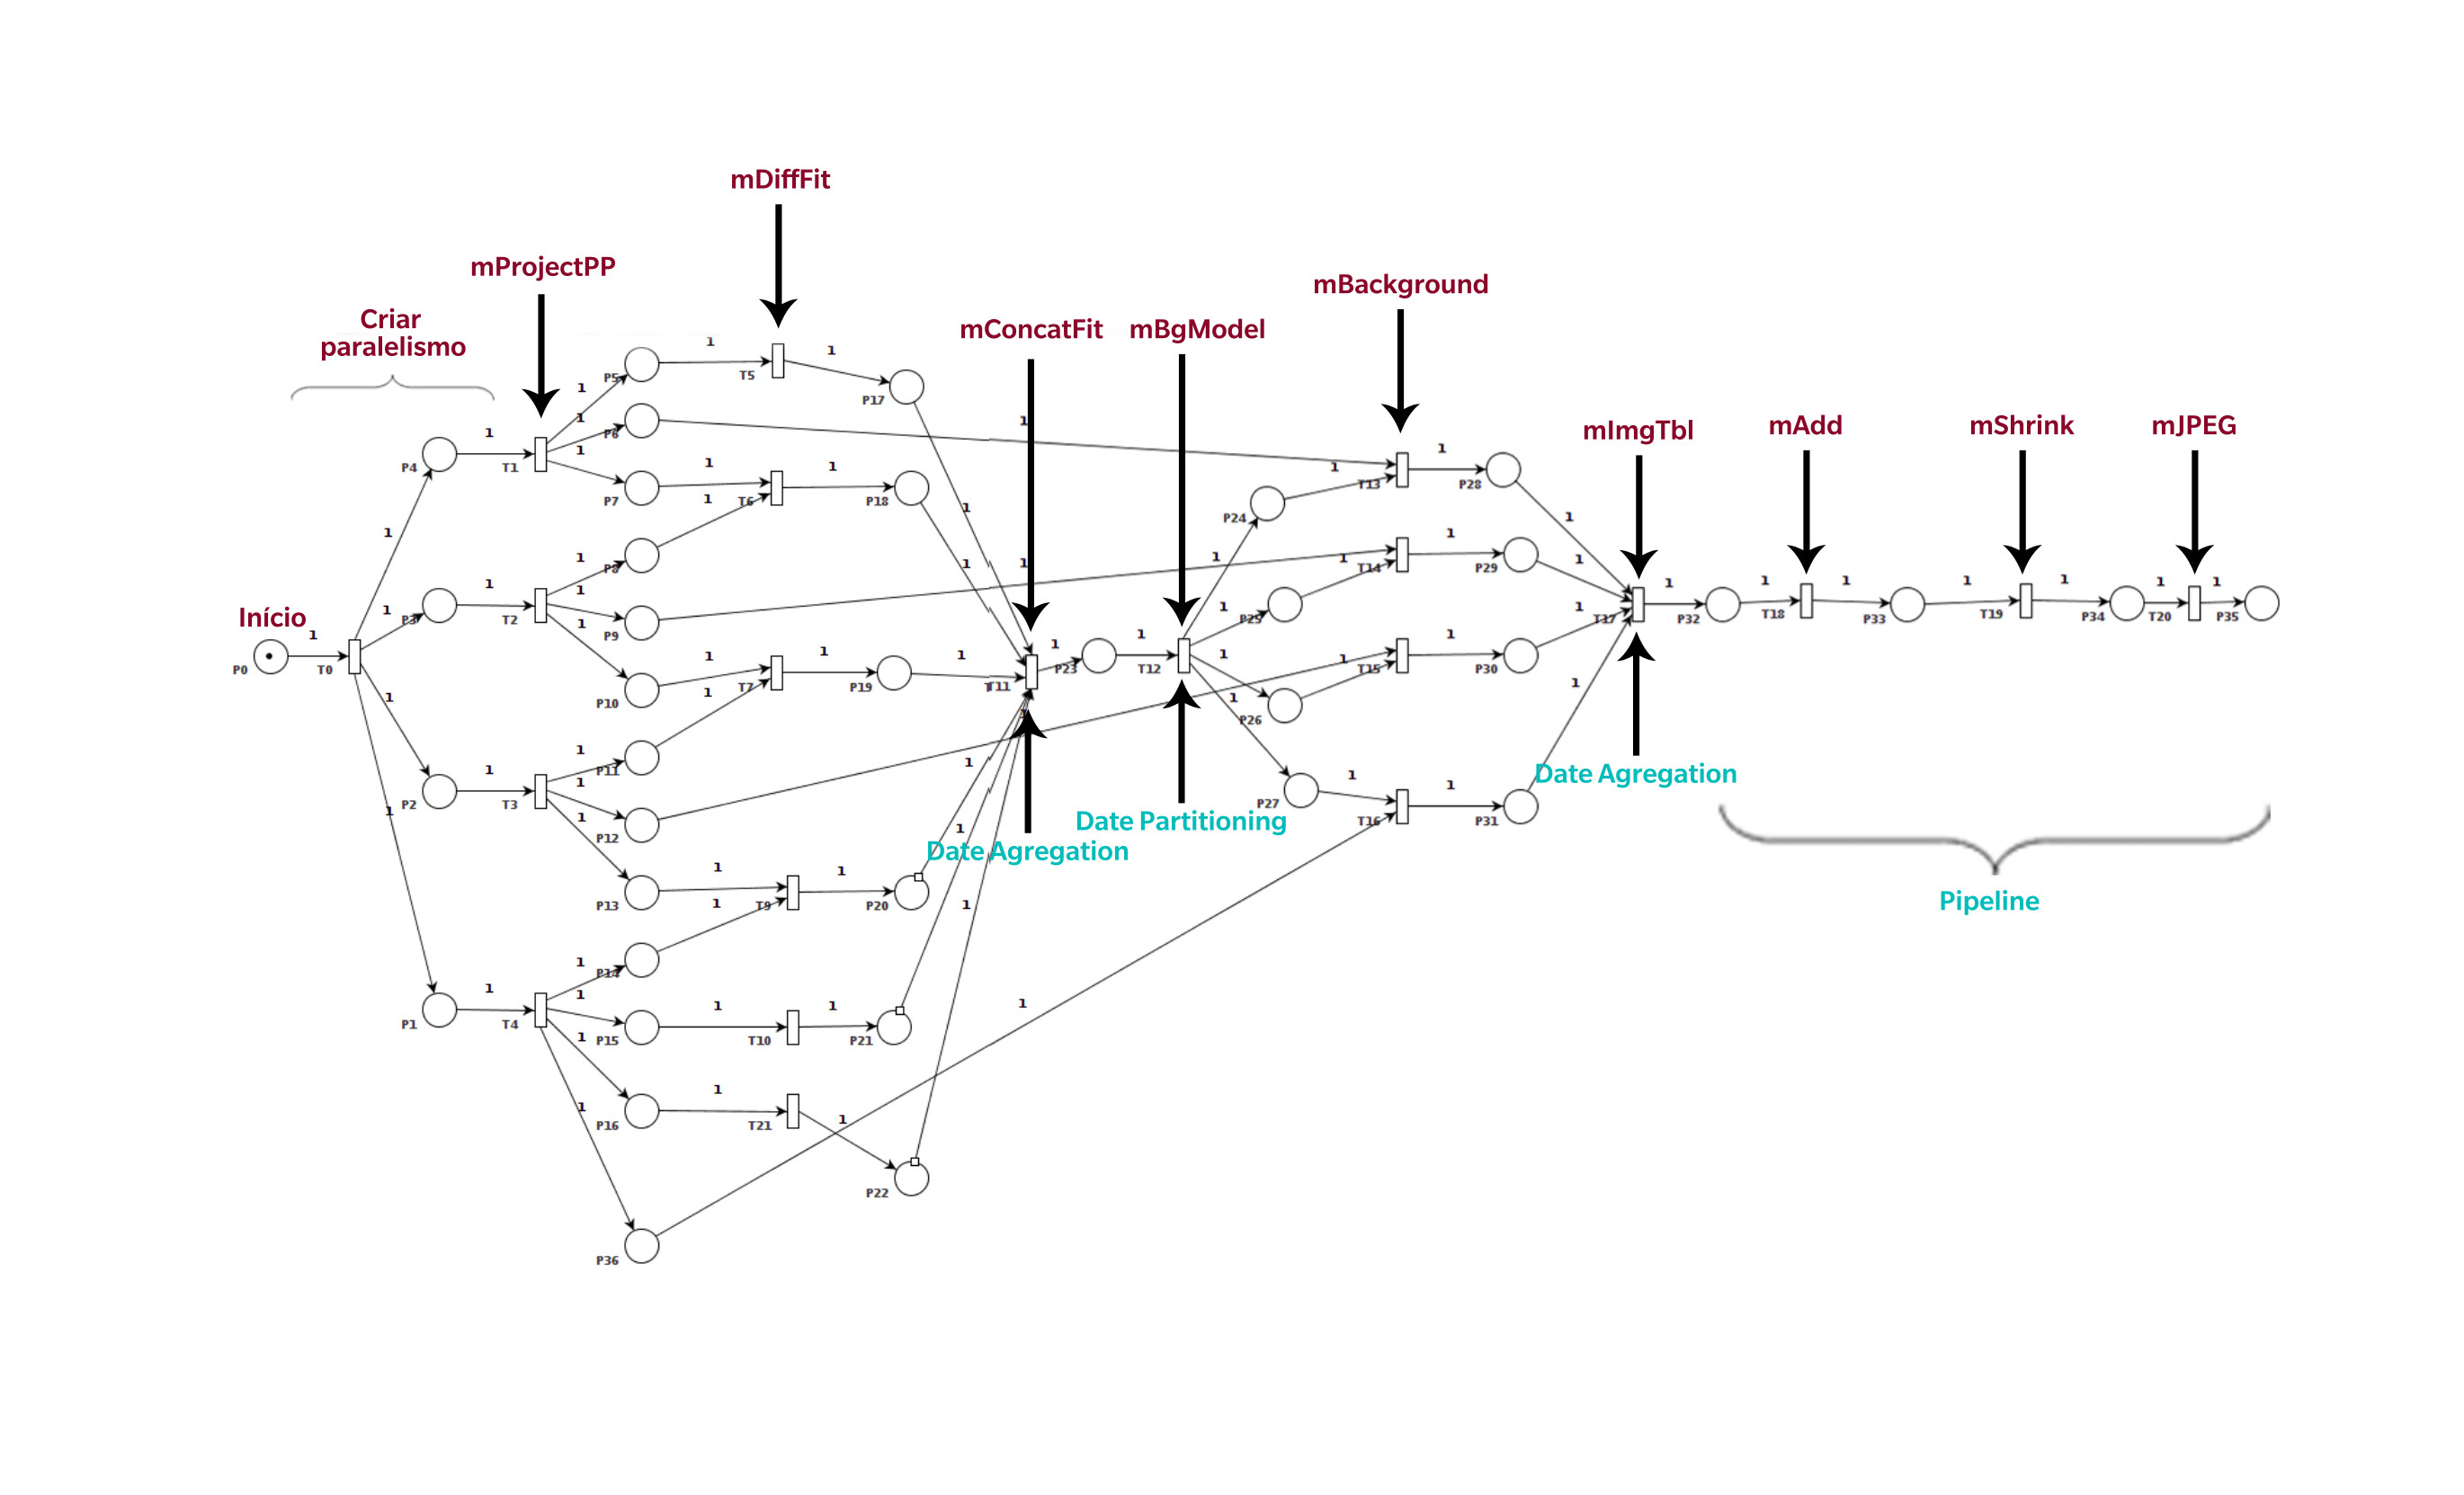
\includegraphics[width=2 \textwidth]{img/RP_montage.jpg}
		\label{Anexo2}
	\end{figure}
\end{landscape}

\subsection{Anexo 3}
\begin{lstlisting}[caption=Descricão de uma ambiente computacional no WorkflowSim]

######Overhead Related Parameters
######The Workflow Engine Delay for level 1
#d1		= 8.1 
######The Workflow Engine Delay for level 2
#d2		= 18.44 
######The Workflow Engine Delay for other levels that are not specified 
#d0		= 6.74
######The Postscript Delay for level 1
#p1		= 78.05
######The Postscript Delay for level 2
#p2		= 13.12
######The Postscript Delay for other levels that are not specified
#p0		= 6.81
######The Queue Delay for level 1
#q1		= 77.75
######The Queue Delay for level 2
#q2		= 343.47
######The Queue Delay for other levels that are not specified
#q0		= 161.96
######The Clustering Delay for level 1
#c1		= 428.28
######The Clustering Delay for level 2
#c2		= 67.44
######The interval for Workflow Engine
#interval	= 5

######Failure related parameters
######The Task Failure Rate for level 1
#a1		= 0.02
######The Task Failure Rate for level 2
#a2		= 0.02
######Fault tolerant clustering method
#ftc.method	= FTCLUSTERING_DC
######Fault tolerant clustering monitor mode
#ftc.monitor	= MONITOR_ALL
######Fault tolerant clustering failure generation mode
#ftc.failure	= FAILURE_JOB

######Clustering Related parameters
######The number of clustered jobs per level
#clusters.num 	= 20
######The size of a clustered job (number of tasks per job)
#clusters.size 	= 20
######The clustering method
#clusters.method = horizontal
#clusters.method = balanced
######The type of file system to use
file.system	= LOCAL
#file.system	= SHARED

######Scheduling Related Parameters
######If you have specified planner.method, it will be disabled
scheduler.method= MINMIN_SCH

######Planning Related Parameters
#planner.method= RANDOM
#deadline = 100000

######Please replace it with your real physical path
dax.path = /home/duilio/workspace/WorkflowSim-1.0-master/config/dax/Montage_1000.xml
######Reducer mode used to remove duplicate dependencies
#reduce.method	= montage
\end{lstlisting}
\label{configworkflowsim}